\section{In-Distribution Forecasting Results}
\label{sec:in_distribution_results}


\subsection{Point Forecasting Performance}
\label{subsec:point_results}

The point forecasting performance of the three models is reported in
Table~\ref{tab:point_results}. For the two probabilistic neural models, the
median prediction $q_{0.5}$ is used as the point forecast. As expected,
forecasting accuracy decreases as the prediction horizon increases, with
both MAE and RMSE increasing from 15 to 60 minutes for all models.

\begin{table}[t]
    \centering
    \caption{Point forecasting performance on the test set at the three
    forecasting horizons. The best result for each metric and horizon is
    highlighted in bold.}
    \label{tab:point_results}
    \begin{tabular}{llccc}
        \toprule
        & & \multicolumn{3}{c}{Forecast horizon} \\
        \cmidrule(lr){3-5}
        Model & Metric & 15 min & 30 min & 60 min \\
        \midrule

        Persistence
        & MAE  & 3.501 & 4.199 & 5.351 \\
        & RMSE & 6.411 & 8.023 & 10.279 \\
        \midrule

        Temporal GRU
        & MAE  & 3.080 & 3.735 & 4.733 \\
        & RMSE & 6.081 & 7.548 & 9.411 \\
        \midrule

        Graph-Temporal
        & MAE  & \textbf{2.901} & \textbf{3.442} & \textbf{4.244} \\
        & RMSE & \textbf{5.511} & \textbf{6.758} & \textbf{8.378} \\
        \bottomrule
    \end{tabular}
\end{table}

The Persistence baseline exhibits the largest errors at all forecasting
horizons. Introducing temporal modeling through the GRU consistently improves
over persistence, showing that the recent history contains temporal patterns
that cannot be captured by simply propagating the final input value into the
future.

The Graph-Temporal model further reduces both MAE and RMSE at every horizon.
Compared with the Temporal GRU, the MAE decreases from 3.080 to 2.901 at
15 minutes, from 3.735 to 3.442 at 30 minutes, and from 4.733 to 4.244 at
60 minutes. These correspond to relative reductions of approximately
5.8\%, 7.8\%, and 10.3\%, respectively. The corresponding RMSE reductions
are approximately 9.4\%, 10.5\%, and 11.0\%.

The improvement introduced by the graph component becomes more pronounced
as the forecasting horizon increases. This suggests that spatial information
is particularly useful for longer-term predictions, where the future state
of a sensor becomes increasingly difficult to estimate from its own temporal
history alone. The reduction in RMSE is also consistently larger than the
reduction in MAE, indicating that the Graph-Temporal model is particularly
effective in reducing larger forecasting errors.

The same trend is illustrated in
Figure~\ref{fig:point_performance}, where the performance gap between the
Temporal GRU and the Graph-Temporal model becomes progressively larger toward
the 60-minute horizon.

\begin{figure}[t]
    \centering

    \begin{minipage}[b]{0.48\linewidth}
        \centering
        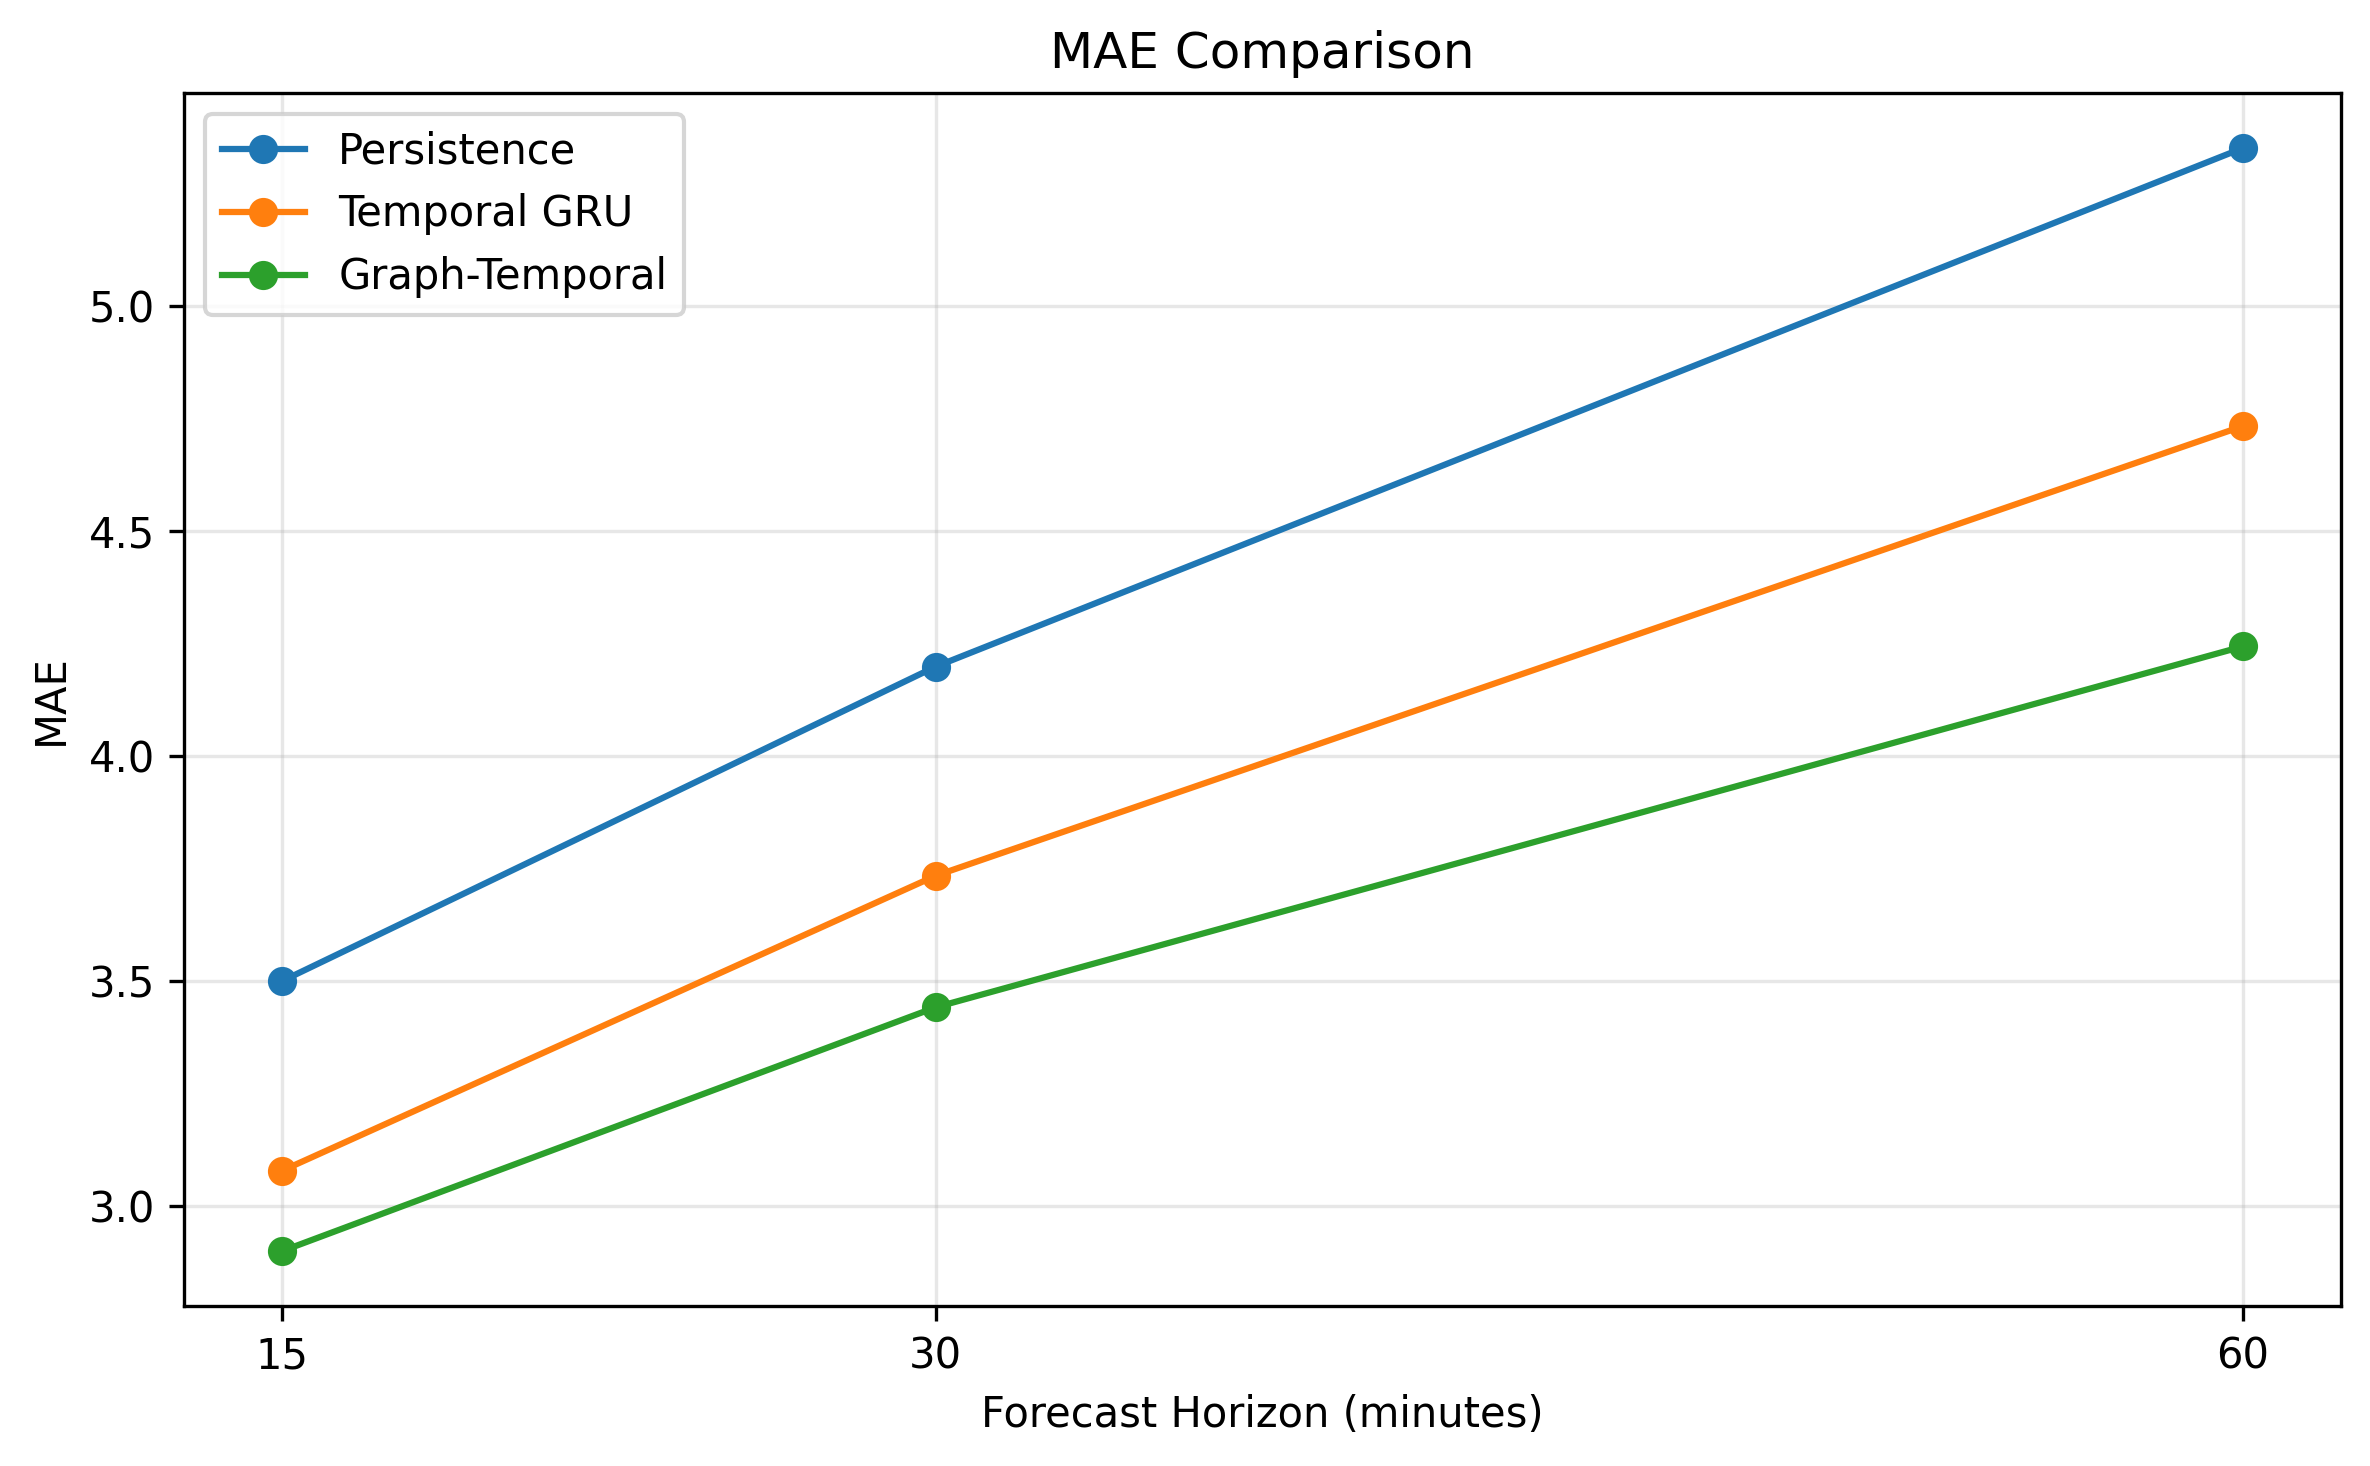
\includegraphics[width=\linewidth]{img/model_comparison/mae_model_comparison}
    \end{minipage}
    \hfill
    \begin{minipage}[b]{0.48\linewidth}
        \centering
        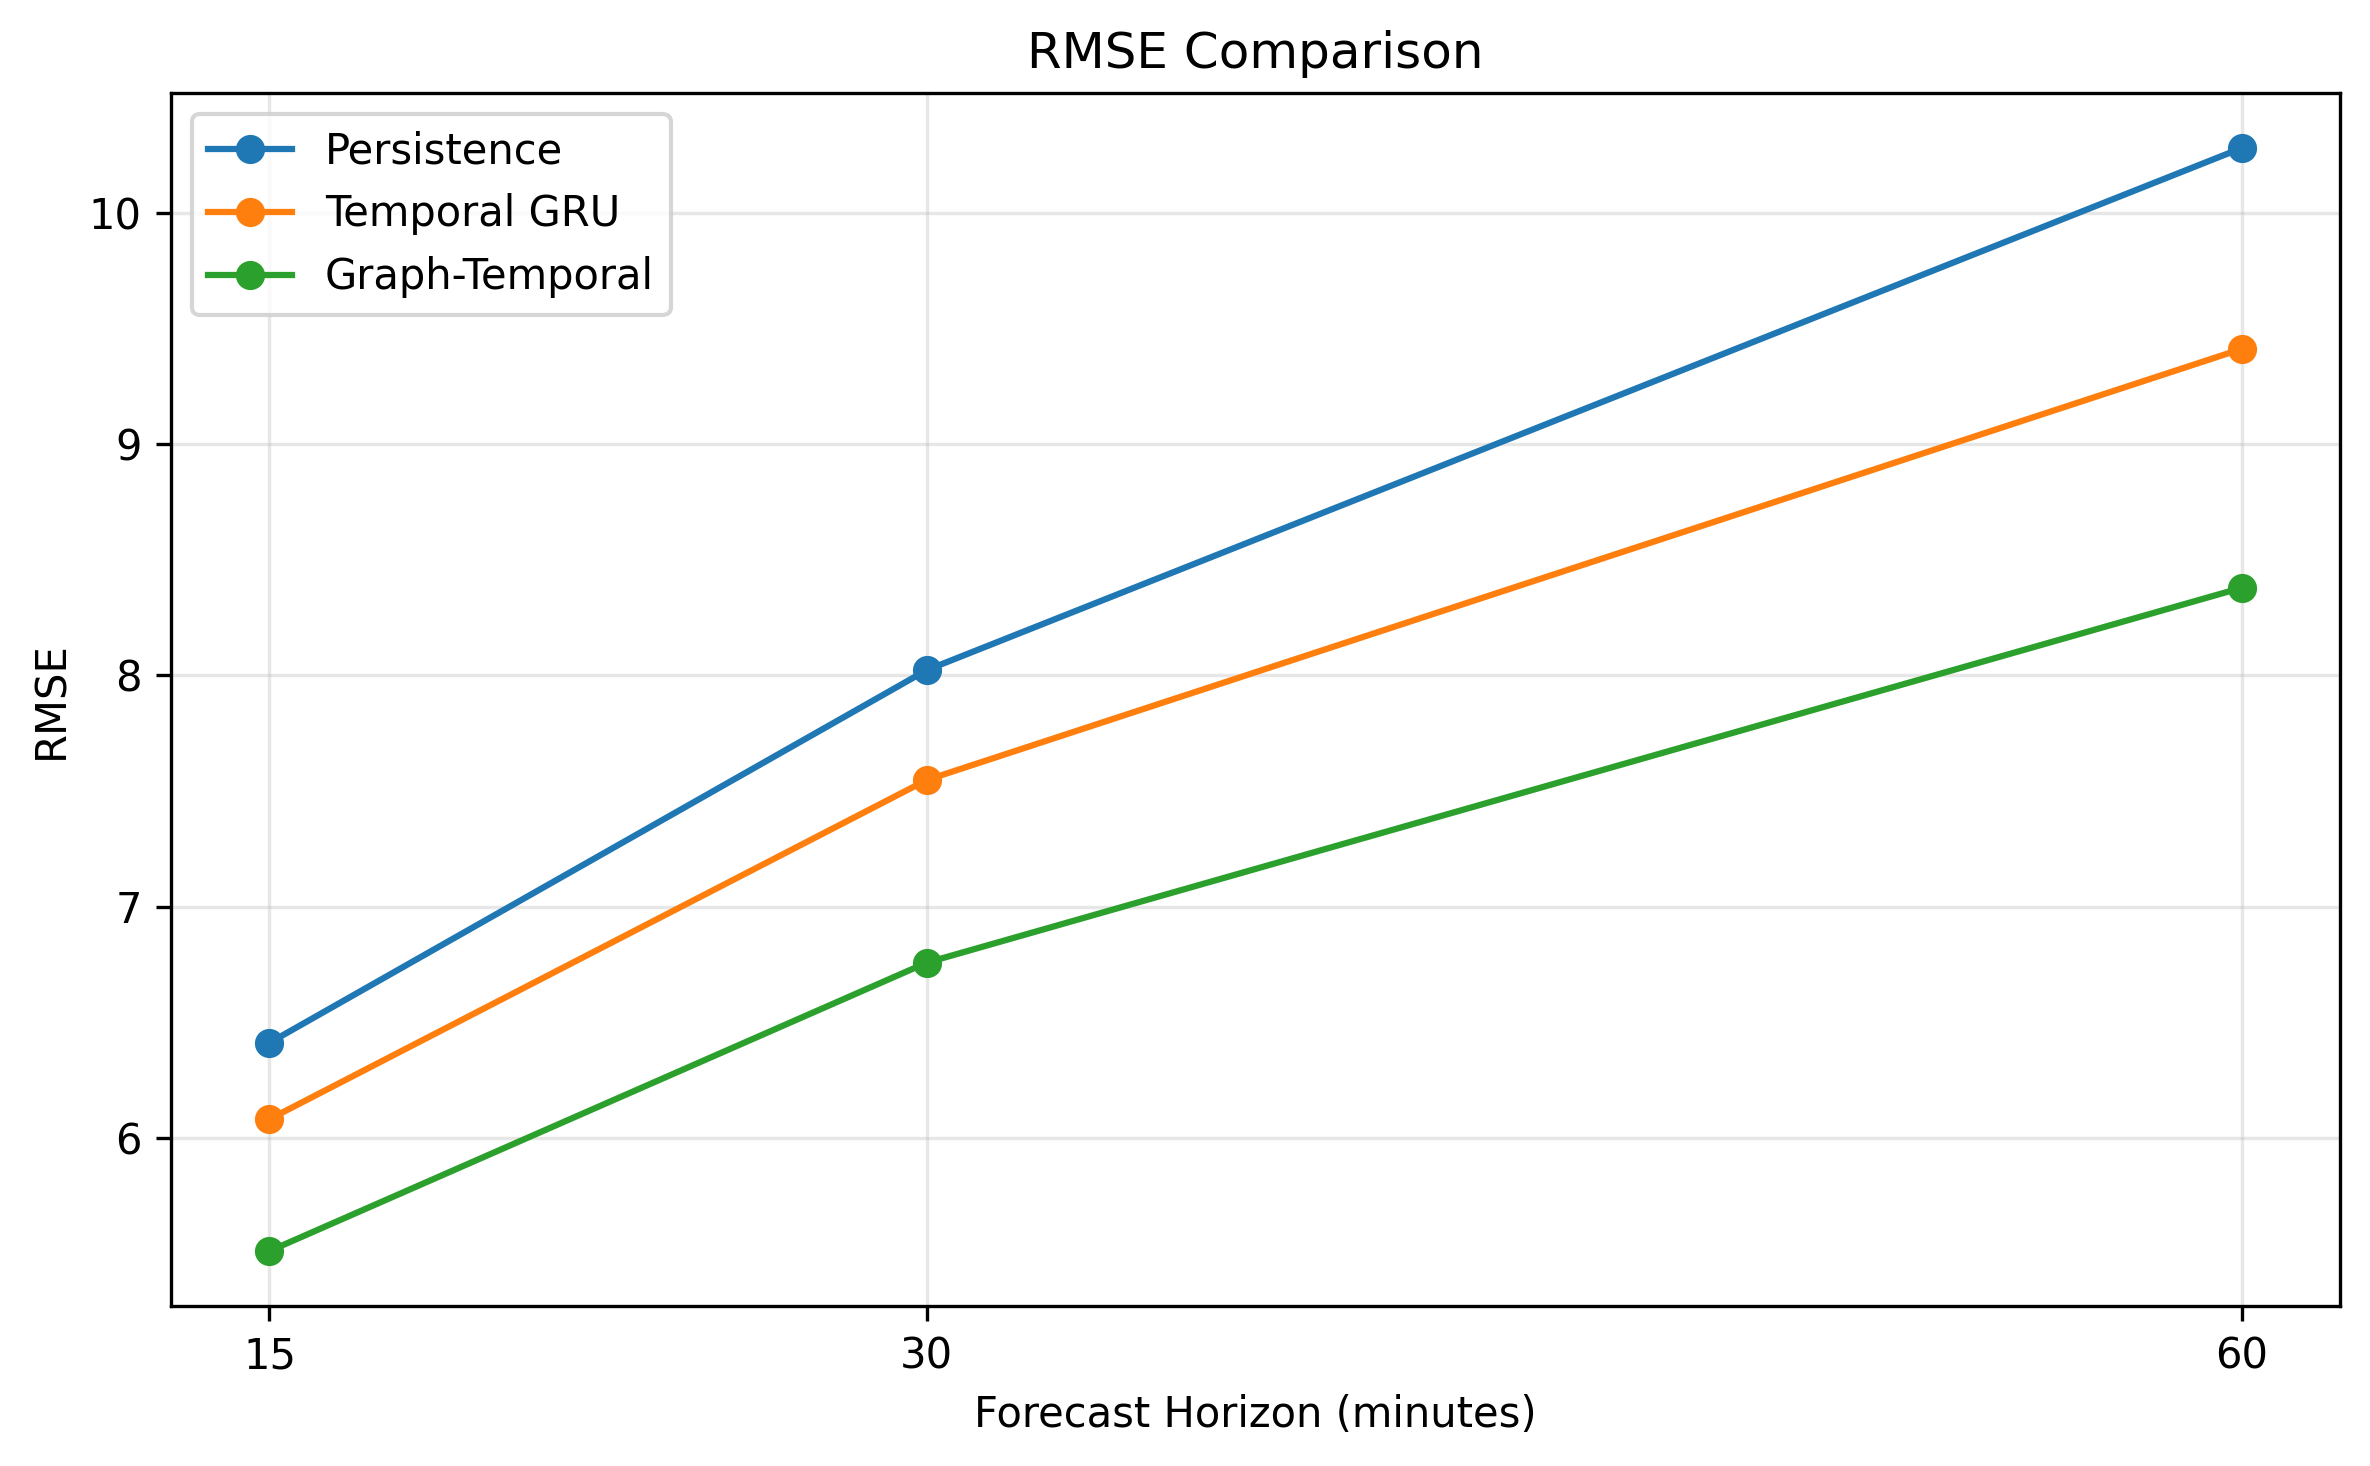
\includegraphics[width=\linewidth]{img/model_comparison/rmse_model_comparison}
    \end{minipage}

    \caption{Point forecasting performance of the Persistence, Temporal,
    and Graph-Temporal models across the three forecasting horizons in terms
    of MAE (left) and RMSE (right).}
    \label{fig:point_performance}
\end{figure}



\subsection{Probabilistic Forecasting and Calibration}
\label{subsec:probabilistic_results}

The probabilistic forecasting performance of the Temporal GRU and
Graph-Temporal models is reported in Table~\ref{tab:probabilistic_results}.
The Pinball Loss is evaluated separately for the three predicted quantiles,
while empirical coverage and interval width are used to assess the reliability
and sharpness of the nominal 80\% prediction intervals.

Across all forecasting horizons, the Graph-Temporal model achieves lower
Pinball Loss for each of the three quantiles. At 15 minutes, the losses for
$q_{0.1}$, $q_{0.5}$, and $q_{0.9}$ decrease from 0.952, 1.540, and 0.643
for the Temporal GRU to 0.845, 1.451, and 0.597 for the Graph-Temporal
model. The same behavior is observed at 30 and 60 minutes, indicating that
the benefit of incorporating spatial information is not limited to the
median forecast, but also extends to the estimation of the lower and upper
quantiles.

The two models, however, exhibit a different trade-off between calibration
and sharpness. The Temporal GRU achieves empirical coverage close to the
nominal 80\% level, with values of 81.30\%, 80.16\%, and 79.81\% at 15,
30, and 60 minutes, respectively. The Graph-Temporal model produces narrower
prediction intervals at every horizon, reducing the average interval width
from 9.339 to 8.929 at 15 minutes, from 10.931 to 10.485 at 30 minutes, and
from 13.309 to 12.470 at 60 minutes. This increased sharpness is accompanied
by slightly lower coverage, which remains between 78.13\% and 78.44\% across
the three horizons.

These results show that the Graph-Temporal model improves the quality of all
three estimated quantiles and produces more concentrated predictive
intervals, but the resulting intervals exhibit mild undercoverage relative
to the nominal 80\% level. In contrast, the Temporal GRU remains closer to
the nominal coverage overall, although it exhibits mild overcoverage at the
15-minute horizon, reaching 81.30\%.
The reliability--sharpness trade-off is further illustrated in
Figure~\ref{fig:probabilistic_comparison}.
Moreover, interval width increases with the
forecasting horizon for both models, reflecting the greater uncertainty of
longer-term predictions. The calibration behavior of the selected
Graph-Temporal model is further investigated under distribution shift in
Section~\ref{sec:distribution_shift}.

\begin{table}[t]
    \centering
    \caption{Probabilistic forecasting performance on the test set. Coverage
    refers to the nominal 80\% prediction interval defined by
    $q_{0.1}$ and $q_{0.9}$.}
    \label{tab:probabilistic_results}
    \resizebox{\linewidth}{!}{
    \begin{tabular}{llccccc}
        \toprule
        Model & Horizon
        & Pinball $q_{0.1}$
        & Pinball $q_{0.5}$
        & Pinball $q_{0.9}$
        & Coverage (\%)
        & Interval Width \\
        \midrule

        Temporal GRU
        & 15 min & 0.952 & 1.540 & 0.643 & 81.30 & 9.339 \\
        & 30 min & 1.225 & 1.867 & 0.743 & 80.16 & 10.931 \\
        & 60 min & 1.668 & 2.367 & 0.832 & 79.81 & 13.309 \\
        \midrule

        Graph-Temporal
        & 15 min & \textbf{0.845} & \textbf{1.451} & \textbf{0.597}
        & 78.44 & \textbf{8.929} \\
        & 30 min & \textbf{1.028} & \textbf{1.721} & \textbf{0.677}
        & 78.22 & \textbf{10.485} \\
        & 60 min & \textbf{1.320} & \textbf{2.122} & \textbf{0.775}
        & 78.13 & \textbf{12.470} \\
        \bottomrule
    \end{tabular}
    }
\end{table}

\begin{figure}[t]
    \centering

    \begin{minipage}[b]{0.49\linewidth}
        \centering
        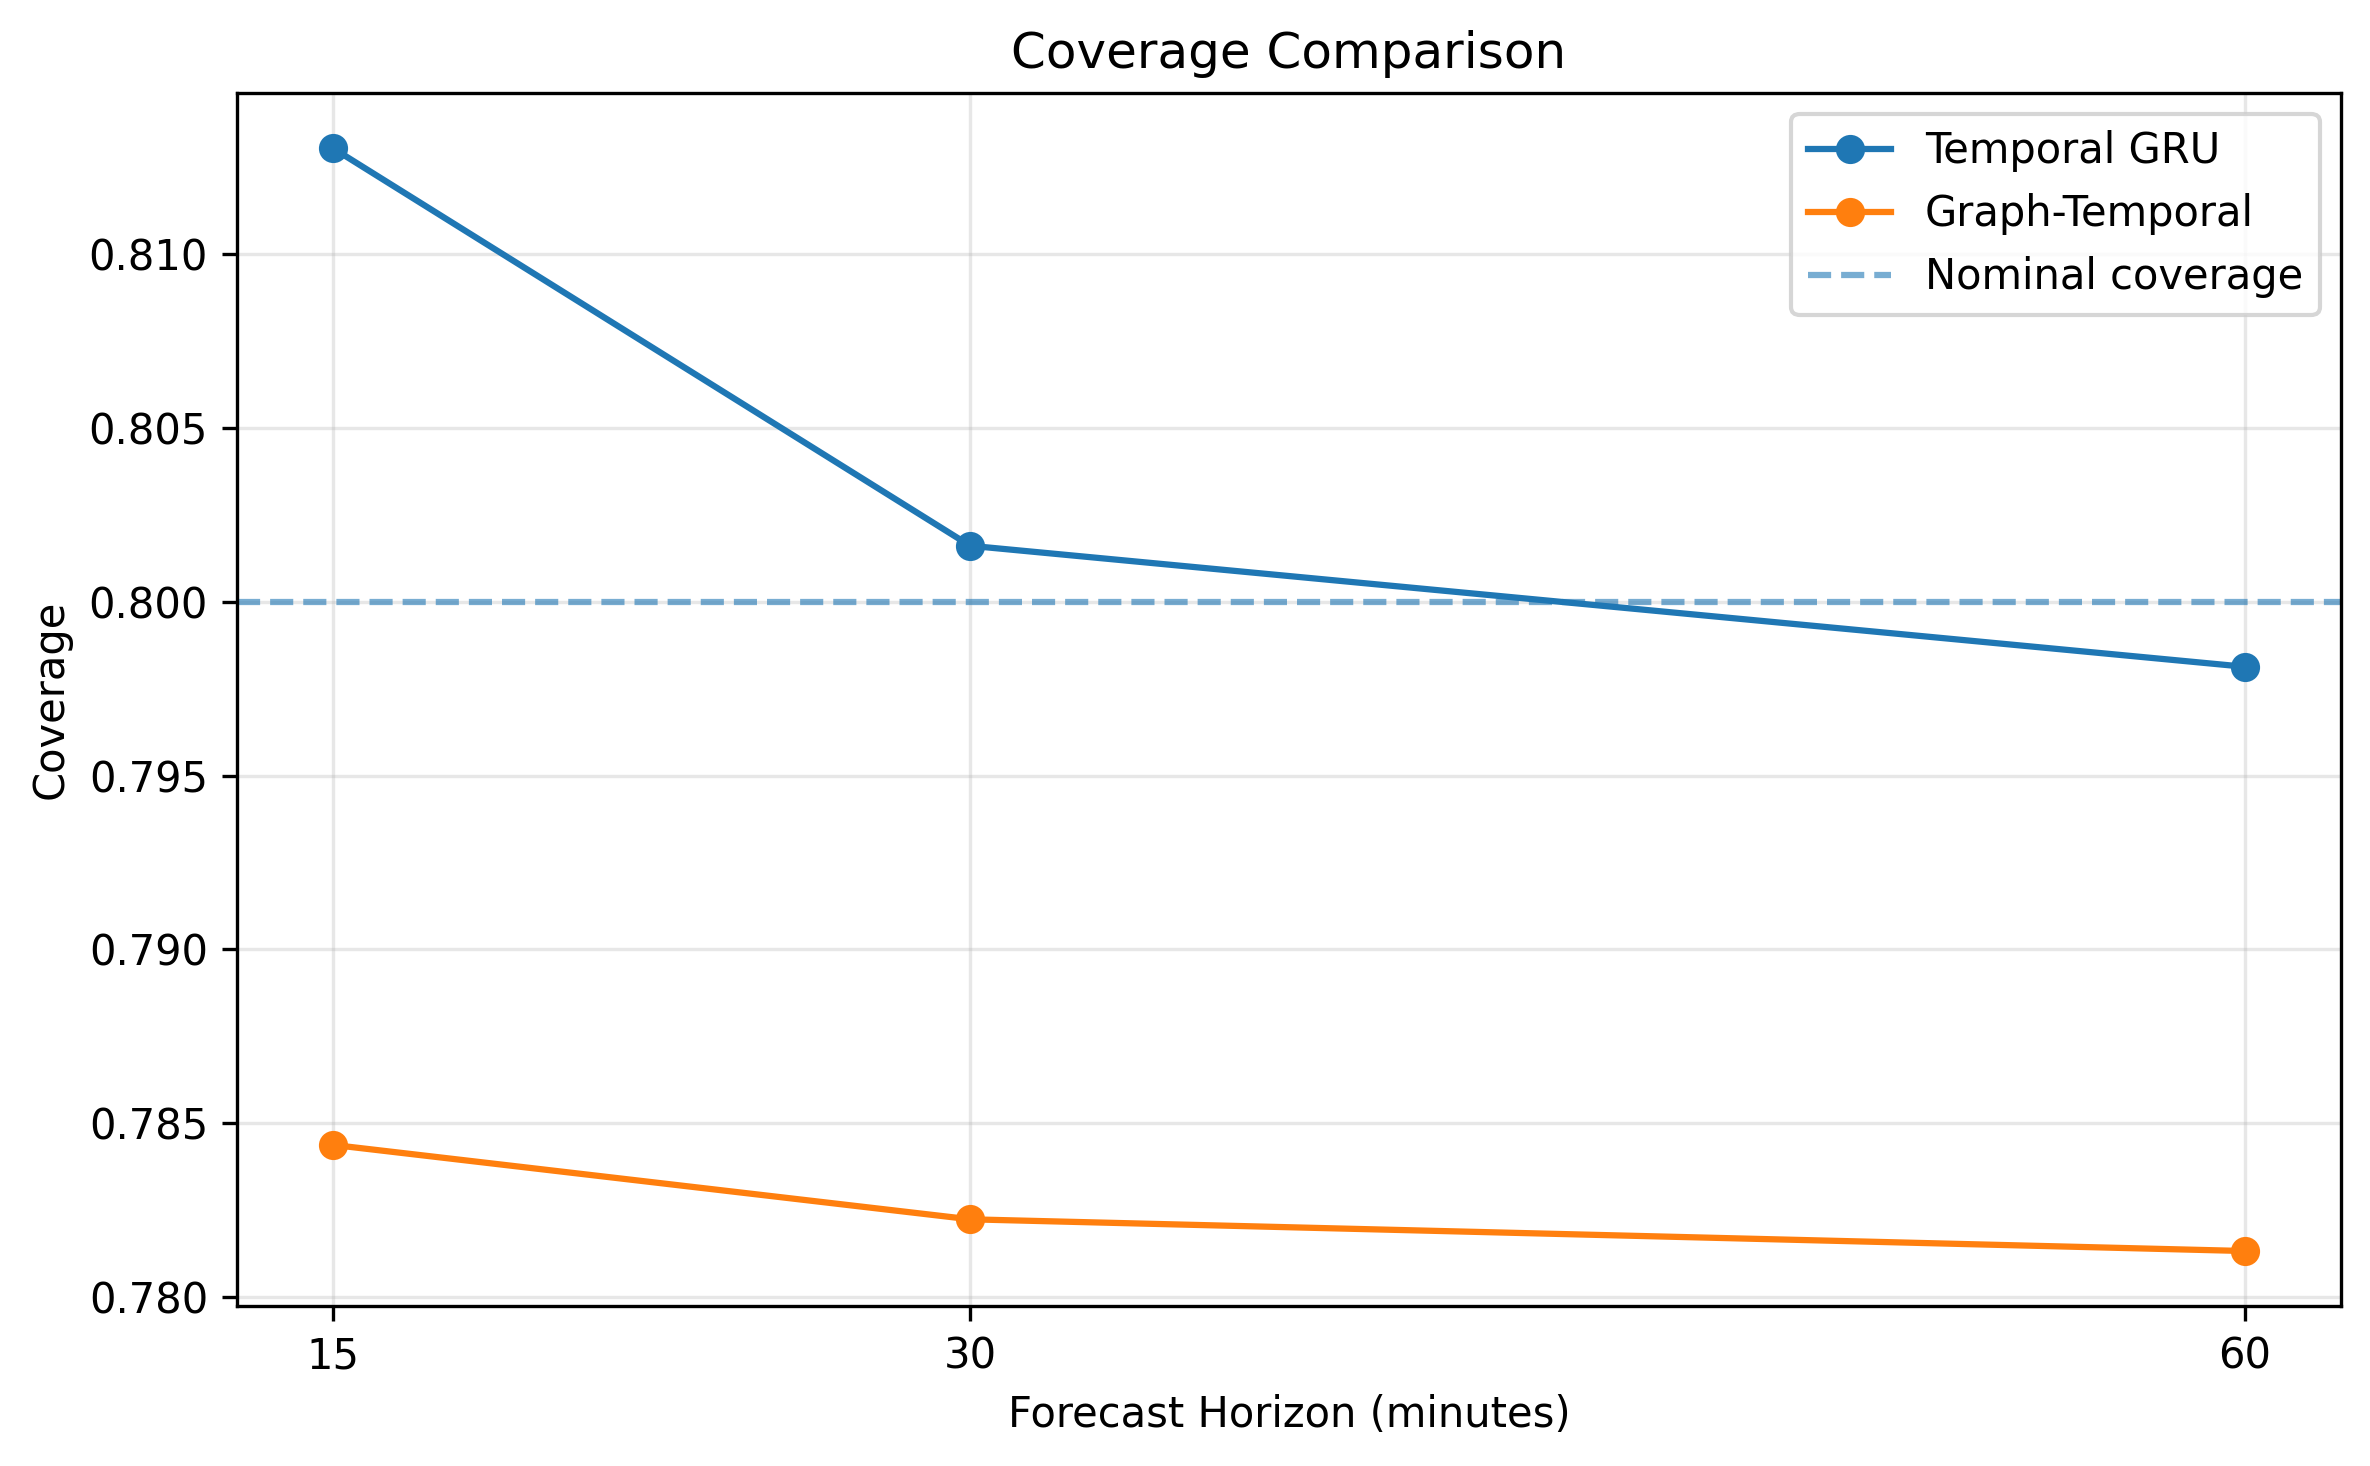
\includegraphics[width=\linewidth]{img/model_comparison/coverage_model_comparison}
    \end{minipage}
    \hfill
    \begin{minipage}[b]{0.49\linewidth}
        \centering
        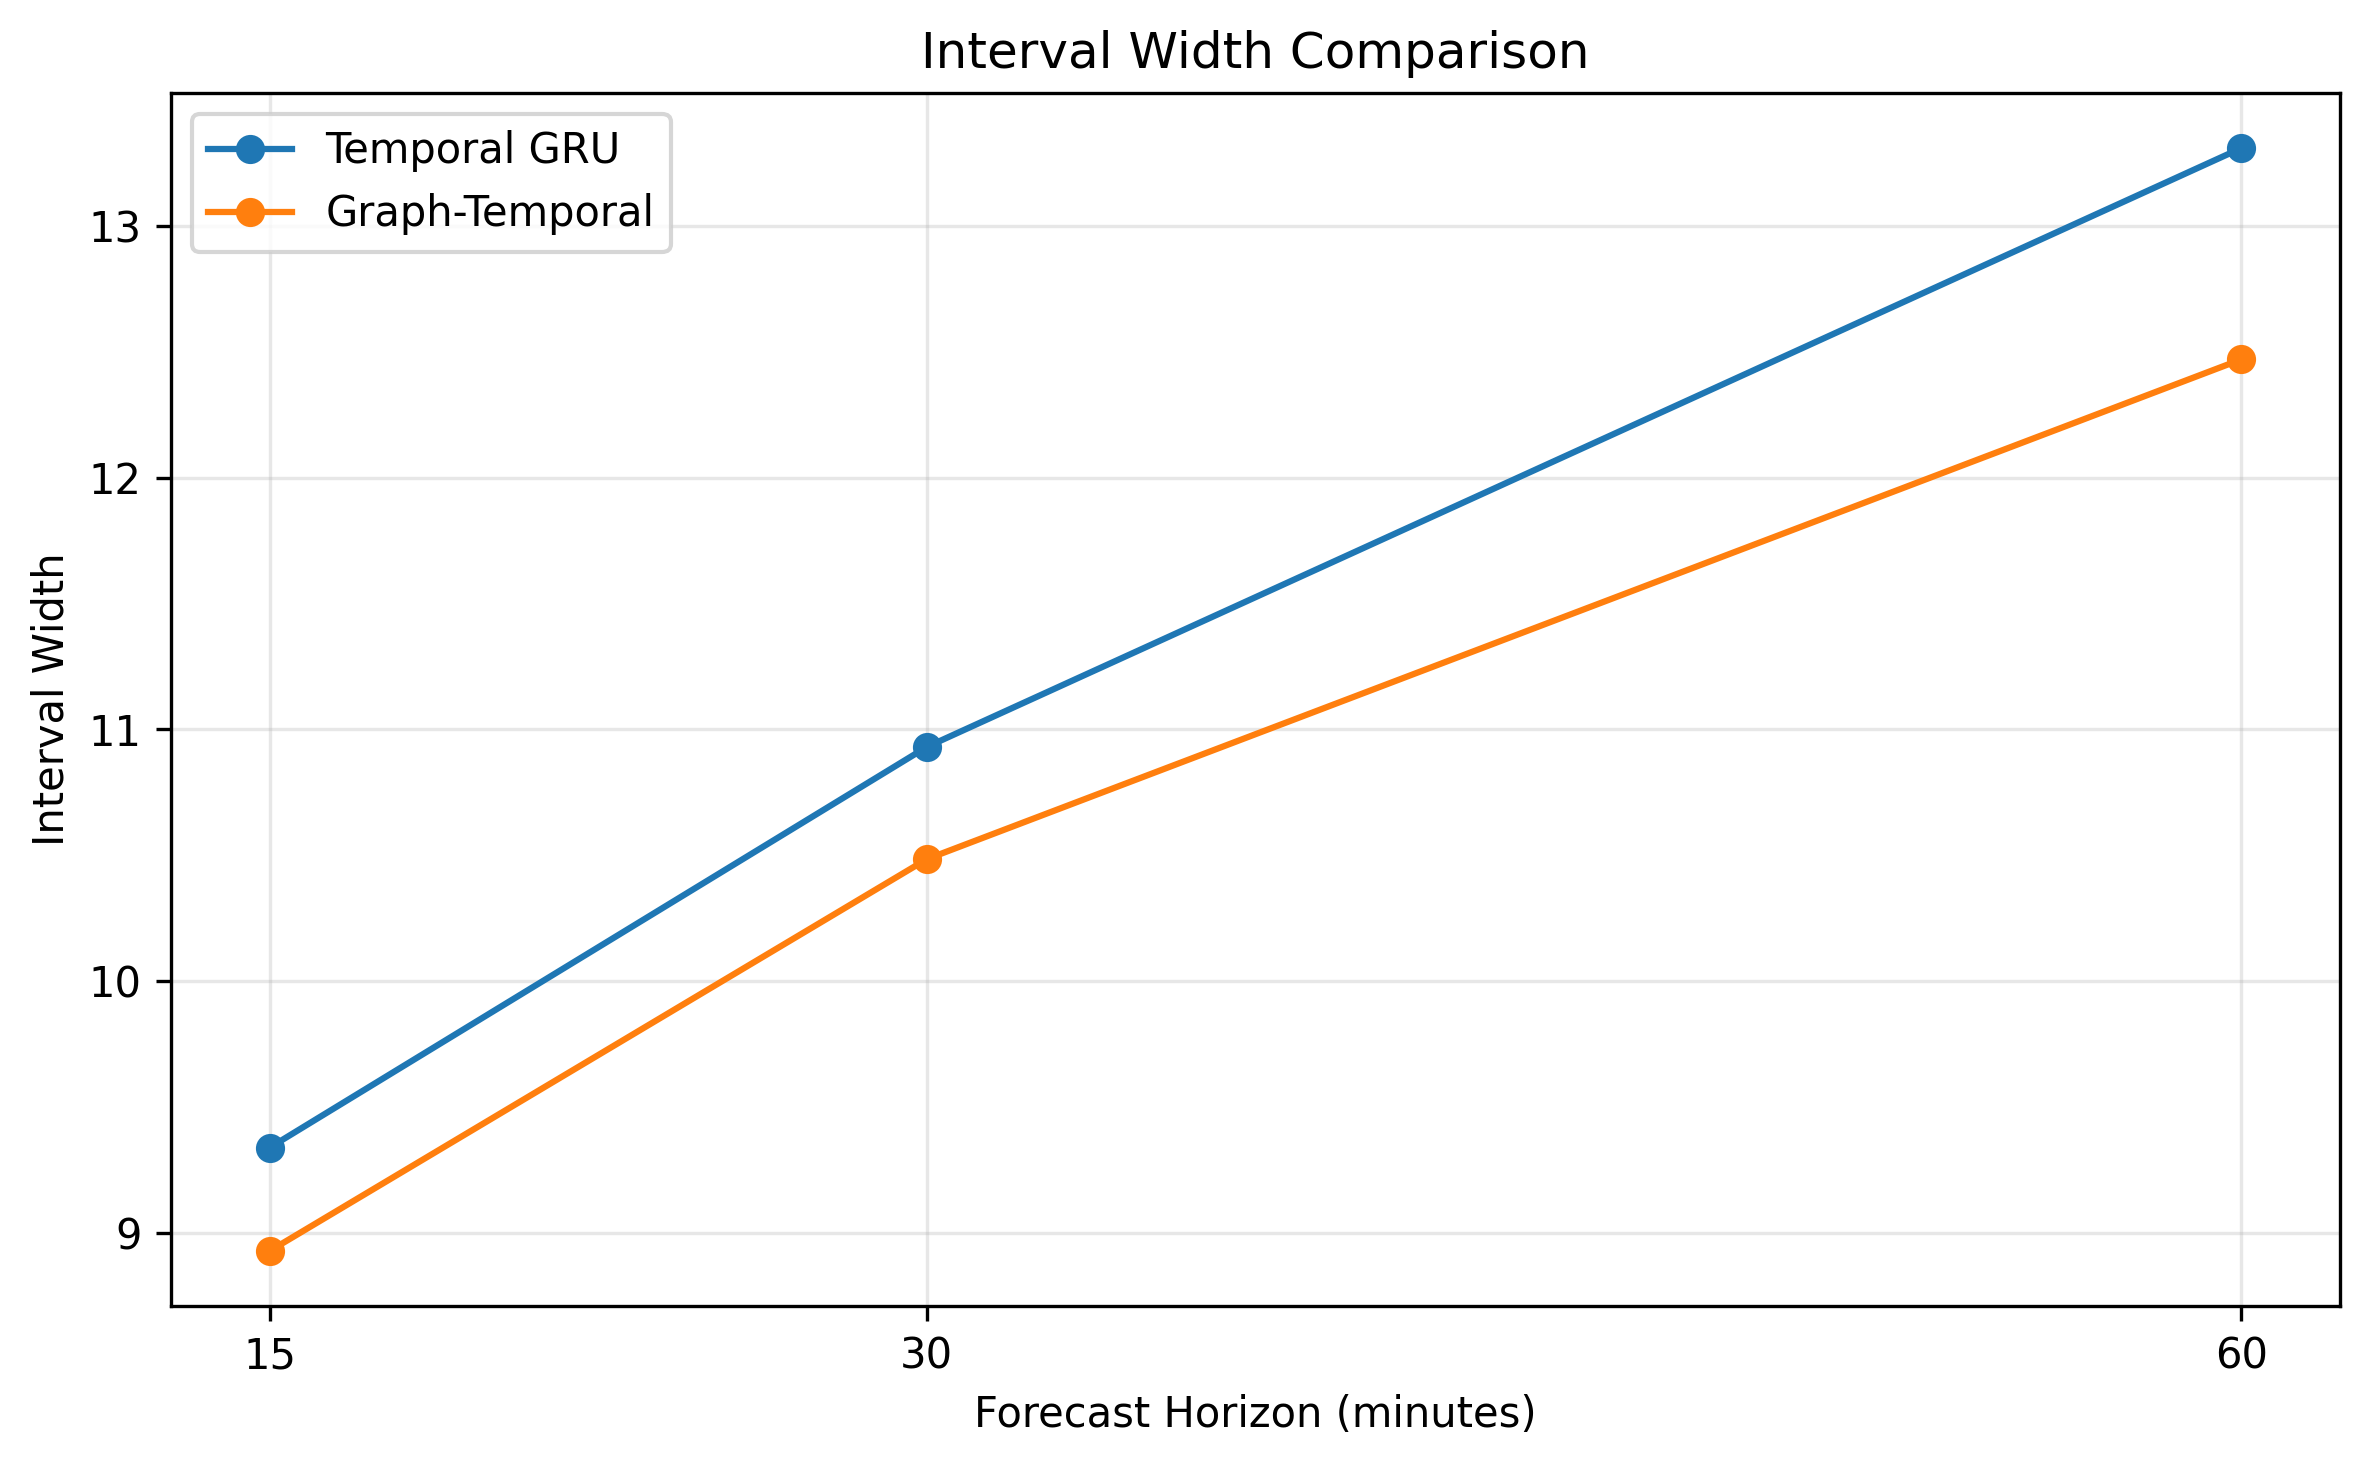
\includegraphics[width=\linewidth]{img/model_comparison/interval_width_model_comparison}
    \end{minipage}

    \caption{Comparison of the probabilistic forecasts produced by the
    Temporal GRU and Graph-Temporal models in terms of empirical coverage
    (left) and prediction interval width (right) across the three forecasting
    horizons. The dashed line in the coverage plot represents the nominal
    80\% coverage level.}
    \label{fig:probabilistic_comparison}
\end{figure}

Quantile crossing is negligible for both models, with rates below 0.05\%
at every forecasting horizon, indicating that the predicted quantiles
almost always preserve their expected ordering.

A more detailed view of probabilistic reliability is provided by the
calibration curves in Figure~\ref{fig:quantile_calibration}. The plots compare the
nominal quantile levels with their empirical frequencies and complement the
interval-level coverage results reported in
Table~\ref{tab:probabilistic_results}.

\begin{figure}[t]
    \centering

    \begin{minipage}[b]{0.49\linewidth}
        \centering
        
\includegraphics[width=\linewidth]{img/temporal_gru/calibration_plot}
    \end{minipage}
    \hfill
    \begin{minipage}[b]{0.49\linewidth}
        \centering
        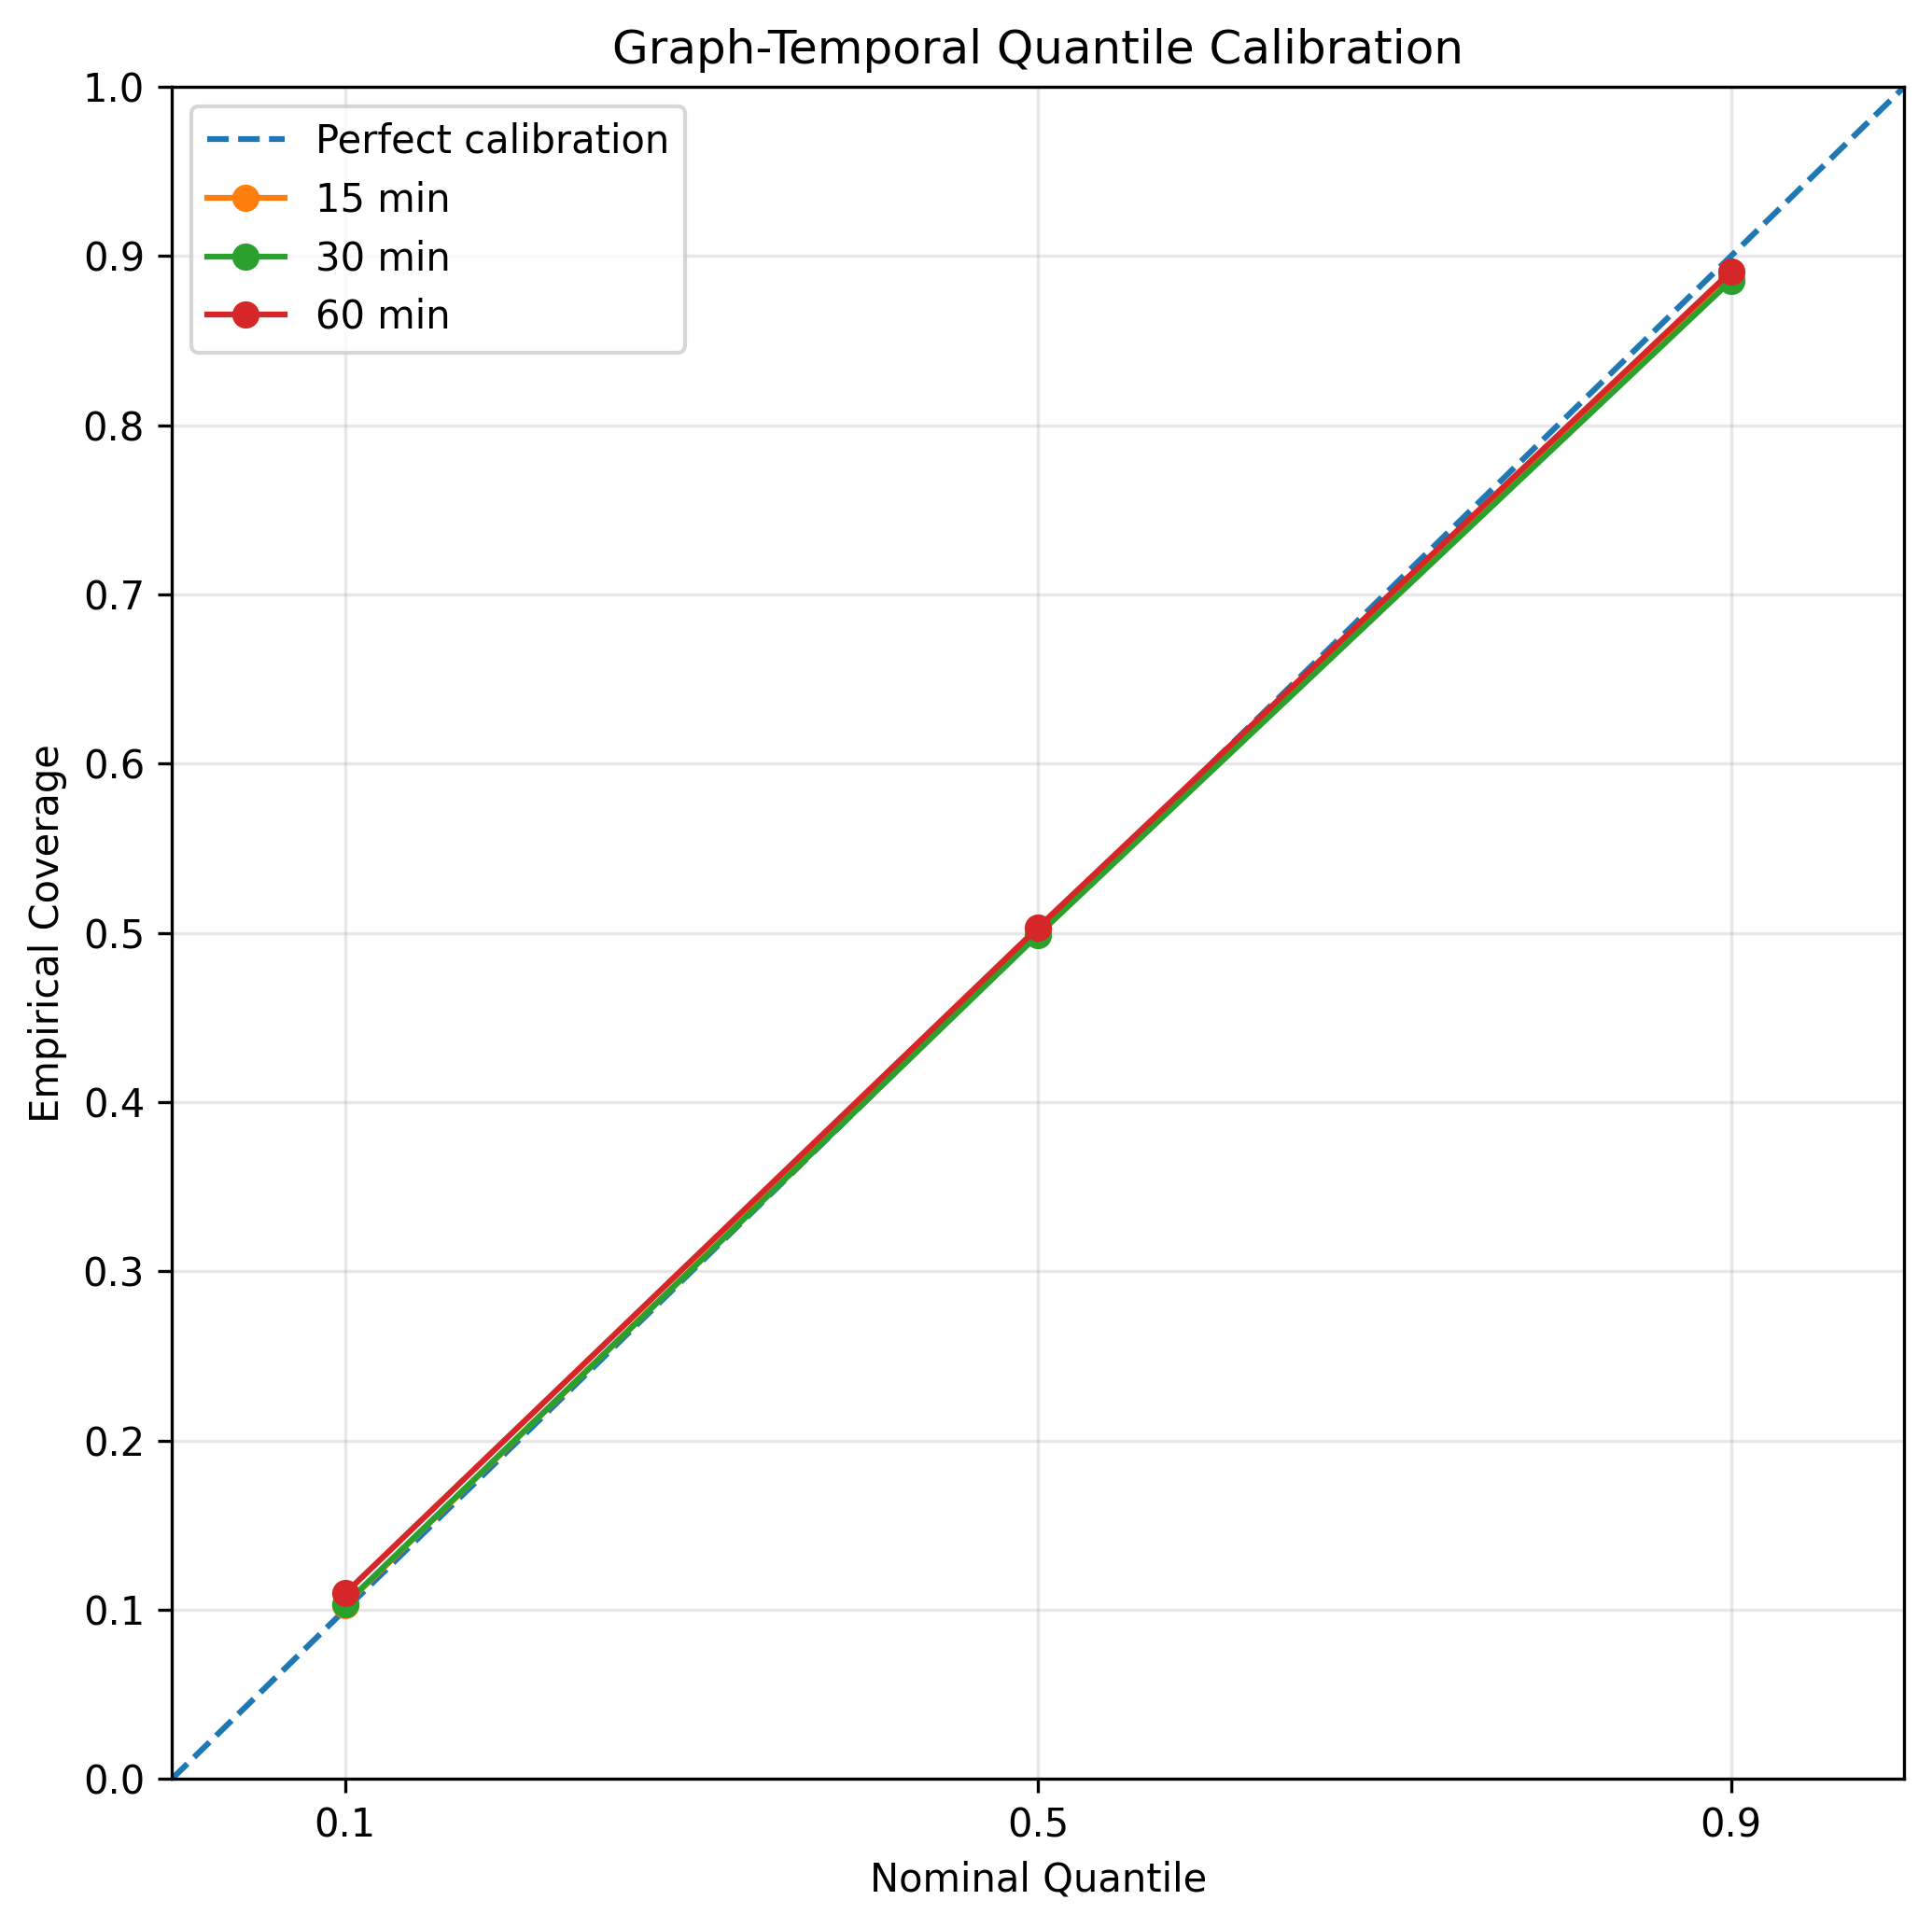
\includegraphics[width=\linewidth]{img/graph_temporal/calibration_plot}
    \end{minipage}

    \caption{Quantile calibration of the Temporal (left) and
    Graph-Temporal (right) models at the three forecasting horizons.
    The dashed diagonal represents perfect calibration.}
    \label{fig:quantile_calibration}
\end{figure}